\documentclass[10pt,twocolumn,letterpaper]{article}

\usepackage{cvpr}
\usepackage{times}
\usepackage{epsfig}
\usepackage{graphicx}
\usepackage{amsmath}
\usepackage{amssymb}
\usepackage{multirow}
\usepackage{graphicx}
\usepackage{subfigure}
\usepackage{caption}

% Include other packages here, before hyperref.

% If you comment hyperref and then uncomment it, you should delete
% egpaper.aux before re-running latex.  (Or just hit 'q' on the first latex
% run, let it finish, and you should be clear).
\usepackage[pagebackref=true,breaklinks=true,letterpaper=true,colorlinks,bookmarks=false]{hyperref}

% \cvprfinalcopy % *** Uncomment this line for the final submission

\def\cvprPaperID{****} % *** Enter the CVPR Paper ID here
\def\httilde{\mbox{\tt\raisebox{-.5ex}{\symbol{126}}}}

% Pages are numbered in submission mode, and unnumbered in camera-ready
\ifcvprfinal\pagestyle{empty}\fi
\begin{document}

%%%%%%%%% TITLE
\title{Bi-Directional Domain Translation for Zero-Shot Sketch-Based Image Retrieval}

\author{First Author\\
Institution1\\
Institution1 address\\
{\tt\small firstauthor@i1.org}
% For a paper whose authors are all at the same institution,
% omit the following lines up until the closing ``}''.
% Additional authors and addresses can be added with ``\and'',
% just like the second author.
% To save space, use either the email address or home page, not both
\and
Second Author\\
Institution2\\
First line of institution2 address\\
{\tt\small secondauthor@i2.org}
}

\maketitle
%\thispagestyle{empty}

\maketitle
%\thispagestyle{empty}

%%%%%%%%% ABSTRACT
\begin{abstract}
   Sketch-Based Image Retrieval (SBIR) is a cross-modal retrieval task, which uses free-hand sketches to retrieve from natural image gallery with the \textbf{same category}. 
   However, SBIR requires all categories can be seen during training, which is not guaranteed. 
   So we investigate a more challenging task, Zero-Shot Sketch-Based Image Retrieval (ZS-SBIR), in which testing categories do not appear at training stage. 
   Traditional SBIR method are prone to be category-based retrieval and cannot generalize well from seen categories to unseen ones. 
   In contrast, we disentangle image feature into structure feature and appearance feature to facilitate structure-based retrieval.
   To realize the function of feature disentanglement and take full advantage of disentangled information, we propose Bi-directional Domain Translation for zero-shot sketch-based image retrieval (BDT) framework, in which the image domain and sketch domain can be translated to each other through disentangled structure and appearance feature.
   Moreover, we also perform retrieval in both structure feature space and image feature space. 
   Extensive experiments demonstrate that our proposed approach remarkably outperforms state-of-the-art approaches by about 8\% on Sketchy dataset and about 5\% on TU-Berlin dataset in the retrieval.
\end{abstract}

\section{Introduction}
%% 1. 多媒体的发展是的image retrieval的主要动力
%% 2. sketch中蕴含着image的形状和形态信息,且容易绘画,所以渐渐变成一个研究热点
%% 3. 传统的设置,假设训练集合和测试集合所拥有的模型是相同的,所以主要关注如何减小sketch的intra-class variance和如何有效利用sketch中的稀疏的信息。经过多年的发展,sbir也取得了很好的效果。
%% 4. 但是这种假设在实际中不存在!
In recent years, with the rapid growth of multimedia data on the internet, the role of image retrieval has become more and more important in many fields, such as remote sensing and e-commerce. 
Since the sketch can be easily drawn and express shape and pose details about the target images, sketch-based image retrieval (SBIR), which use a sketch to retrieve images with the same category, has become widely accepted among users. 
Therefore, SBIR has also attracted widespread attention in the research community \cite{del1997visual, cao2010mindfinder, eitz2010evaluation, eitz2010sketch, cao2011edgel, hu2011bag, zhou2012sketch, hu2013performance, cao2013sym, parui2014similarity, james2014reenact, wang2015sketch, saavedra2015sketch, li2016fine, yu2016sketch, qi2016sketch, sangkloy2016sketchy, lu2018learning}. 
In the conventional setting, it is assumed that the images and sketches in training and testing set share the same categories.
However, in real-world applications, the categories of test sketches/images may be out of the scope of training categories.

%% 1. 本文主要研究zero-shot情况下的这一问题
%% 2. 前人的研究已经证明,在这种情况下,传统的模型并不能取得很好的效果,这主要是因为因为评价指标的导向会使得模型更加倾向于学习基于类别的检索方式,而这种情况并不存在于zero-shot的情况下。
%% 3. zs情况下主要的的问题是如何提升将模型从seen domain泛化到unseen domain。
In this paper, we investigate a more challenge task called zero-shot sketch-based image retrieval (ZS-SBIR), which assure that the test categories do not appear at training stage. 
It has been shown that the performance of existing methods will decline dramatically at ZS-SBIR setting \cite{yelamarthi2018zero}, which probably because existing methods are prone to learn category-based retrieval.
Specifically, since the evaluation methodology is category-based, traditional SBIR methods may take a shortcut by correlating sketches/images with their category labels and retrieving the images from the same category as the query sketch \cite{yelamarthi2018zero}, which is very effective when testing data share the same categories as training data. 
However, they often fail when the testing categories have never been seen at training stage.

\begin{figure}
\begin{center}
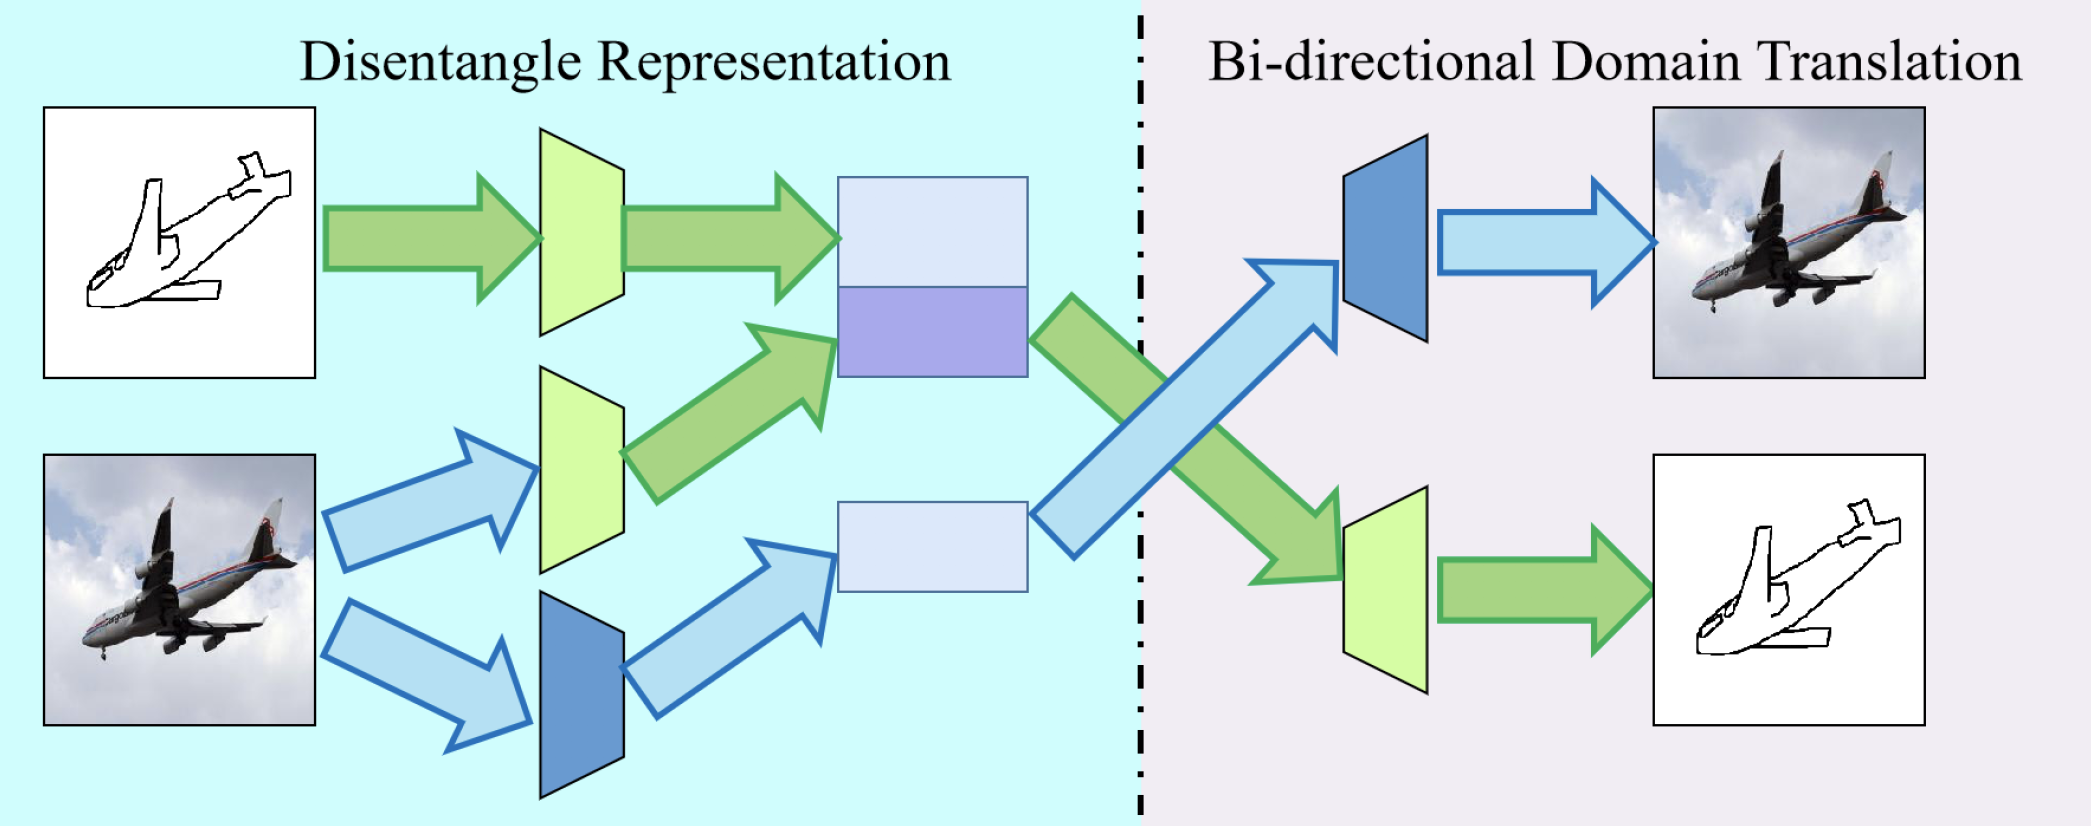
\includegraphics[width=1\linewidth]{modelinshort.png}
\end{center}
   \caption{The overall structure of our model}
\label{fig:inshort}
\end{figure}

%% 1. 为了解决这个问题,一些人尝试使用生成式模型和pose对应的数据来增强模型在seen和unseen domain之间的泛化能力; 一些人尝试使用semantics信息来减小sketch的intra-class bias; 一些人尝试使用semantics的信息来引导同类别sketch和image的correspondence或保留预训练模型中的关键信息。; 
%% 2. 但是pose对应的数据并不容易得到,同时使用semantics信息也难以使得模型的脱离class-based retrieval.(第二点理由应该再重新组织一下)
%% 3. 与他们不同,我们打算将模型的变为倾向于基于结构特征的检索模型。\
To generalize well from seen categories to unseen categories, a model should learn to align  the structure information of sketches with the corresponding structure information of images, which is referred to as structure-based retrieval.
Existing methods for ZS-SBIR can be categorized into three groups, 
(1) some works use generative model based on aligned data pairs, where image and sketch have same shape and pose, to reduce the gap between seen and unseen categories \cite{yelamarthi2018zero}; 
(2) some works use semantic information to reduce the intra-class variance in sketch to stabilize the training process \cite{xu2019semantic, wang2019stacked, dutta2019semantically, shen2018zero}; 
(3) some works fine-tune the pre-trained model in ZS-SBIR task, with semantic-aware knowledge preservation to prevent catastrophic forgetting \cite{liu2019semantic}. 
However, the aligned data pairs and semantic information is not always available. Moreover, all the above methods did not achieve the goal of structure-based retrieval. 
Apart from the methods designed for ZS-SBIR, some prior works tend to generate structure information based on sketch tokens, which are obtained by directly extracting the outlines of image \cite{liu2017deep, wang2015sketch, yu2016sketch}. However, the sketch tokens obtained in this way are not very reliable due to lots of noisy and redundant information, which limits the performance of these methods.
Different from them, we disentangle structure feature from image feature to facilitate structure-based retrieval.

%% 为了达到这个目的,我们设计了一个利用disentangle的方式,将模型的structure信息和appearance信息进行分离,使得模型可以学习到structure-based retrieval,同时,为了更好的将image disentangle之后的appearance information充分利用起来,我们提出了bi-directional domain translation的模型,同时提出了新的retrieval指标。 
As is known to all, sketch is only an outline of image, so we can disentangle the image feature into structure-features and appearance-features, where the structure-features corresponding to the structure information of outlines and the appearance-feature corresponding to additional detailed information, like background and color. 
To realize the function of feature disentanglement and take full advantage of disentangled information, we propose Bi-directional Domain Translation for zero-shot sketch-based image retrieval (BDT) framework, in which sketch and image are treated as two domains. 
As shown in Figure \ref{fig:structure}, we first use a pre-trained model (e.g., VGG) to extract features from sketches and images, which are referred to as sketch features and image features respectively. 
Then, two independent encoders and and an orthogonal loss are adopted to disentangle the image features into structure features and appearance features.
Sketch feature is also projected to the same structure feature space. 
Then, bi-directional domain translation is performed through these features.
For image-to-sketch translation, we use the image structure features to directly generate the sketch feature. 
For sketch-to-image translation, we adopt an image generator to reconstruct image feature based on both sketch feature and appearance feature, where the latter is used to compensate the uncertainty during generating the image features from sketch features.
Due to the need of stochastic sampling, a variational estimator is adopted to image appearance feature before it combine with sketch structure feature. 
Moreover, we also perform retrieval in both structure feature space and image feature space. 
The overall model and the new retrieval strategy is verified by the quantitative experimental results. 

Our main contributions of this paper are summarized as follow:
\begin{itemize}
	\item To our best knowledge, we are the first to disentangle image feature into structure feature and appearance feature, to facilitate structure-based retrieval.
	\item We propose a bi-directional domain translation framework for zero-shot sketch-based image retrieval task.
	\item Experimental results on two popular large-scale datasets show that our approach significantly outperforms state-of-the-art methods.
\end{itemize}

\section{Related Work}

\subsection{SBIR and ZS-SBIR}
The main goal of sketch-based image retrieval (SBIR) is to build a bridge between image domain and sketch domain. Basically, the methods to solve this problem can be categorized into hand-crafted features based and deep-learned features based. Before deep learning was introduced to this task, hand-crafted based methods mostly work by extracting the edge map from natural image and then matching them with sketch using different Bag-of-Words model on specifically designed feature \cite{saavedra2015sketch, hu2013performance, eitz2010sketch, hu2011bag, eitz2010evaluation}. In recent year, deep learned based methods become popular in this area. To reduce the gap between image domain and sketch domain, variant of siamese networks \cite{qi2016sketch, sangkloy2016sketchy, song2017deep} and ranking losses \cite{chopra2005learning, sangkloy2016sketchy} are adopted to this task. Besides, semantics information and adversarial loss are also introduced to preserve the domain invariant information \cite{chen2018deep}.

The zero-shot sketch-based image retrieval is proposed by \cite{shen2018zero} and then followed by \cite{yelamarthi2018zero, xu2019semantic, wang2019stacked, liu2019semantic, dutta2019semantically}. To reduce the intra-class variance in sketch and stabilize the training process, semantic information is leveraged in \cite{wang2019stacked, shen2018zero, xu2019semantic, dutta2019semantically}. To reduce the gap between seen and unseen categories, generative model along with aligned data pairs is proposed in \cite{yelamarthi2018zero}. To adapt the pre-trained model to ZS-SBIR without forgetting the knowledge of ImageNet \cite{deng2009imagenet}, semantic-aware knowledge preservation mechanism is used in \cite{liu2019semantic} to prevent the catastrophic forgetting.

\subsection{Disentangled Representation}
The disentangled representation is to divide the latent representation into multiple units, with each unit corresponding to one latent factor (e.g., the pose feature can be disentangled from face recognition images \cite{tran2017disentangled}). Each unit is only affected by its corresponding latent factor, but not influenced by other latent factors.

Disentangled representation is more generalizable and semantically meaningful, and thus useful for a variety of tasks.
These methods can be categorized into unsupervised learning and supervised learning.
For the unsupervised disentanglement, it includes InfoGAN \cite{chen2016infogan}, MTAN \cite{liu2018multi}, $\beta$-VAE \cite{higgins2017beta}, JointVAE \cite{dupont2018learning}, FactorVAE \cite{kim2018disentangling}, InfoVAE \cite{zhao2017infovae} and TCVAE \cite{chen2018isolating}. 
In this manner, the most common approach first define the prior over the latent variables with a fully-factorized Gaussian distribution and use the prior to encourage the feature disentanglement in different dimensions of the latent representation.
For the second part, Kingma \textit{et al.}  \cite{kingma2014semi} first use disentangled representation to enhance the semi-supervised learning. Zheng \textit{et al.} \cite{zheng2019joint} propose DG-Net to integrate discriminative and generative learning using disentangled representation. Besides, the effectiveness of supervised disentanglement in different applications, like person re-id \cite{zheng2019joint}, face recognition \cite{liu2018unified, liu2018exploring, shu2017neural, tran2017disentangled} and image generation \cite{ma2018disentangled, yan2016attribute2image, mathieu2016disentangling, jha2018disentangling} also helps to attracted great attention.

\subsection{Domain Translation}
Many domain translation approaches, like Pix2Pix \cite{pix2pix2017}, CycleGAN \cite{zhu2017unpaired}, BiCycleGAN \cite{zhu2017toward}, StarGAN \cite{StarGAN2018}, DiscoGAN \cite{kim2017learning} have been proposed, which can translate figures between different domains (e.g., sketch domain and image domain).
In this subsection, we mainly discuss the domain translation methods based on disentangled representation. 
They disentangle latent representation into domain-specific representation and domain-invariant representation. 
In our problem, structure feature can be treated as domain-invariant representation and appearance feature can be treated as domain-specific feature.
DRIT \cite{lee2018diverse} and DRIT++ \cite{lee2019drit} use the disentangled representation with VAE to enrich the diversity during inference. MUNIT \cite{huang2018multimodal} and CDD \cite{gonzalez2018image} combine the disentanglement objective into image-to-image translation between two domains \color{red} and the disentangled representation also help the model to capture domain-specific and domain-invariant information while generating the images, which is similar to our method. \color{black}

In this paper, we introduce disentangled representation into ZS-SBIR tasks along with a bi-directional domain translation model to take full advantage of disentangled information.


\begin{figure*}
\begin{center}
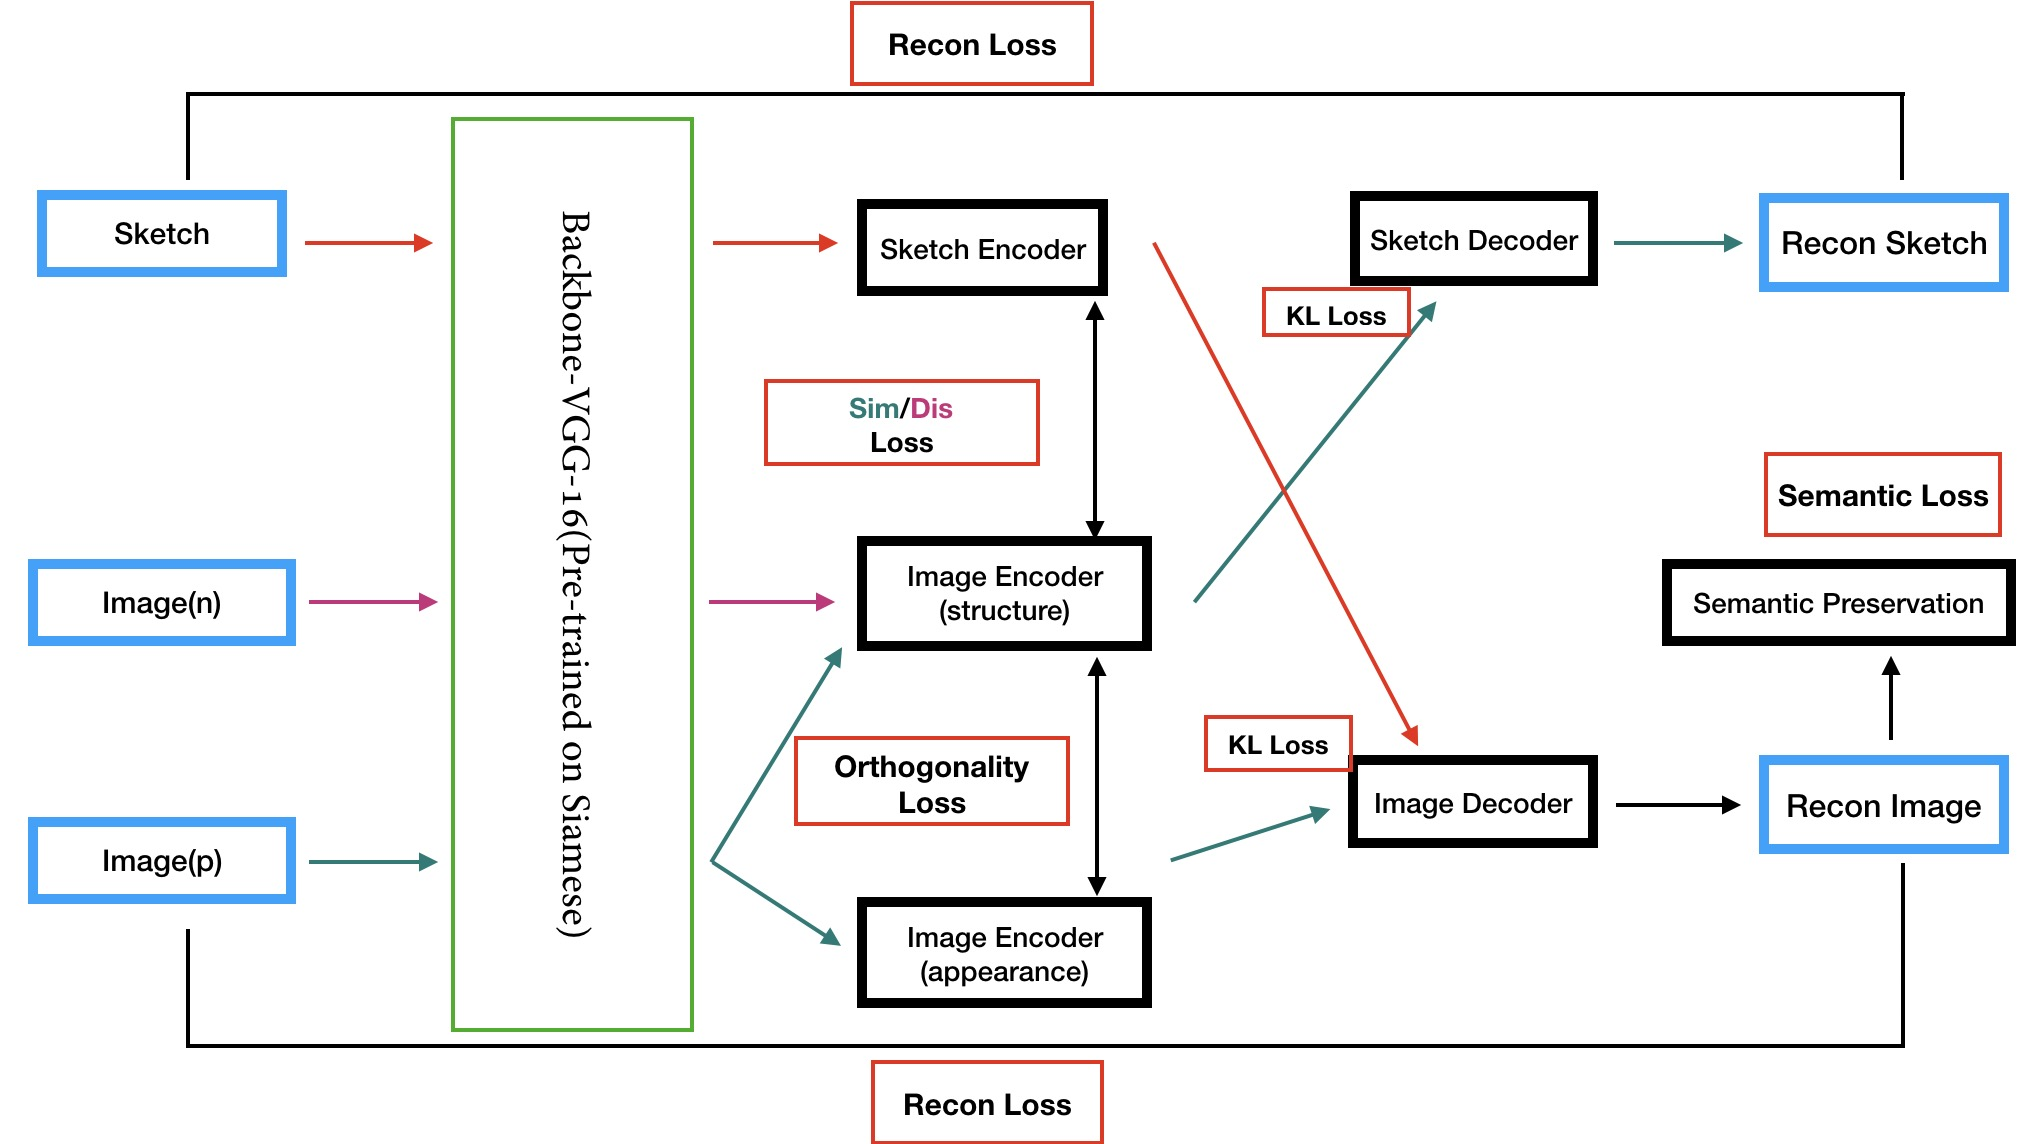
\includegraphics[width=0.95\linewidth]{model_structure.pdf}
\end{center}
   \caption{Model Structure}
\label{fig:structure}
\end{figure*}

\section{Methodology}
In this section, we introduce our proposed Bi-directional Domain Translation for zero-shot sketch-based image retrieval (BDT) framework. In Sec \ref{3.1} we state the problem of ZS-SBIR and define some notations in this paper. In Sec \ref{3.2}, we elaborate the disentangled representation and the bi-directional domain translation modules in detail. In Sec \ref{3.3} we discuss the strategy during training and retrieving.

\subsection{Problem Definition} \label{3.1}
In this paper, we focus on solving the problem of hand-free sketch-based image retrieval under zero-shot setting, where only the sketches and images from seen categories are used at training stage. 
At the testing stage, our proposed framework is expected to use the sketches to retrieve the images, the categories of which have never appeared during training.

We first provide a definition of the SBIR in zero-shot setting. 
Given a sketch dataset $S_{sk}=\{(x_i^{sk}, y_i)|y_i \in \mathcal{Y}\}$ and an image dataset $S_{im}=\{x_j^{im}, y_j | y_j \in \mathcal{Y}\}$, where $(x_i^{sk}, y_i)$ and $(x_j^{im}, y_j)$ are corresponding to the image, sketch and their corresponding category labels.
Following the zero-shot setting in \cite{yelamarthi2018zero,wang2019stacked}, we split all categories $\mathcal{Y}$ into $\mathcal{Y}_{train}$ and $\mathcal{Y}_{te}$, where no overlap exists between two label set, i.e. $\mathcal{Y}_{tr} \cap \mathcal{Y}_{te} = \emptyset$. Considering that we use ImageNet pre-trained model to extract images/sketches feature. To avoid the test category shown at training stage, we also require the testing category not in ImageNet.
Based on the partition of label set $\mathcal{Y}$, we can split sketch (resp., image) dataset into $S^{tr}_{sk}$ and $S^{te}_{sk}$ (resp., $S^{tr}_{im}$ and $S^{te}_{im}$)
At training stage, our model can only process the data in $S^{tr}_{sk}$ and $S_{im}^{tr}$. 
During test, given a sketch $s^{sk}$ from $S^{te}_{sk}$, our model need to retrieve images belonging to the same category as $s^{sk}$ from test images gallery $S^{te}_{im}$.

The overall framework of our method is illustrated in Figure \ref{fig:structure}.
Let $f_{im} \in \mathbb{R}^n$ be the image feature, $f_{sk} \in \mathbb{R}^n$ be the sketch feature, $f^{st}_{im} \in \mathbb{R}^m$ be the image structure feature, $f^{ap}_{im} \in \mathbb{R}^m$ be the appearance feature, $z^{ap}_{im}$ be the variational appearance feature and $f^{st}_{sk} \in \mathbb{R}^m$ be the sketch structure feature. 
Our bi-directional domain translation model builds several feature maps among these features. Before the translation, we first adopt feature extractor to map the image/sketch to their corresponding feature. Two image encoder is applied to disentangle the image feature into structure and appearance features. Meanwhile, the sketch feature is also projected into structure space. For the image-to-sketch translation, the image structure feature is directly translated into the sketch feature. Whereas, for the sketch-to-image translation, we combine the sketch structure feature and the image appearance feature together to get the image feature.
%\color{red}
%Let $f_{im} \in \mathbb{R}^n$ be the image feature, $f_{sk} \in \mathbb{R}^n$ be the sketch feature, $f^{st}_{im} \in \mathbb{R}^m$ be the image structure feature, $f^{ap}_{im} \in \mathbb{R}^m$ be the appearance feature, $z^{ap}_{im}$ be the variational appearance feature and $f^{st}_{sk} \in \mathbb{R}^m$ be the sketch structure feature. 
%Our model consists of a feature extractor $F$, two structure encoders $\{E_{im}^{st}, E_{sk}\}$, one appearance encoder $\{E_{im}^{ap}\}$, one variational estimator $\{V_{im}^{ap}\}$, two domain generators $\{G_{im}, G_{sk}\}$ and two discriminators $\{D_{im}, D_{sk}\}$. 
%$F$ map image/sketch to their corresponding feature space. 
%$E_{im}^{st}$ and $E_{sk}$ map the image feature and sketch feature onto a shared structure feature space, while the $E_{im}^{ap}$ maps the image feature to the appearance feature space. $V_{im}^{ap}$ estimate the variational distribution $Q(z_{im}^{ap}|f_{im}^{ap})$, to support the variational inference during the retrieving, $G_{im}$ generates image features from encoded image structure and $G_{sk}$ generates sketch features conditional on both variational image appearance feature and encoded sketch structure. The discriminators are trained to distinguish the generated images/sketches from the real ones.

%Given these components of our model, we can define the bi-directional domain translation. The sketch to image translation is defined as $\hat{f_{img}} = G_{img}(E_{ske}(f^{ske}), V_{img}^{ap}(E_{img}^{ap}(f^{img})))$. And the image to sketch translation is defined as  $\hat{f_{ske}} = G_{ske}(E_{img}^{st}(f^{img}))$ extract the image structure features from image feature and translate them into sketch features. \color{black}
%\begin{table}[]
%\small
%\begin{tabular}{l|l}
%\hline
%Module                             & Configuration                                                               \\ \hline
%$E_{img}^{ap}$ & FC1;BatchNorm;ReLU;Dropout;FC2;BatchNorm;ReLU                               \\
%$E_{img}^{st}$ & FC1;BatchNorm;ReLU;Dropout;FC2;BatchNorm;ReLU                               \\
%$E_{ske}$                         & FC1;BatchNorm;ReLU;Dropout;FC2;BatchNorm;ReLU                               \\
%$V_{img}^{ap}$ & \begin{tabular}[c]{@{}l@{}}Mean: FC; Tanh\\ Variance: FC; Tanh\end{tabular} \\
%$G_{img}$                         & FC1;ReLU;FC2;ReLU                                                           \\
%$G_{ske}$                         & FC1;ReLU;FC2;ReLU                                                           \\
%$D_{img}$                         & FC1;BatchNorm;ReLU;Dropout;FC2;ReLU                                         \\
%$D_{ske}$                         & FC1;BatchNorm;ReLU;Dropout;FC2;ReLU                                         \\ \hline
%\end{tabular}
%\caption{The detailed configuration of our model}
%\label{table:1}
%\end{table}

\subsection{BDT} \label{3.2}

\subsubsection{Feature Extractor} 
Since sketches are highly abstract and possess intrinsic visual sparsity compared with natural images, it is hard to extra to get more information from the pre-trained model. To alleviate this problem without adding more parameters, we use the feature fusion network in \textit{Wang et al.} \cite{wang2019stacked} and concatenate the features extracted from multiple layers of the pre-trained model to get the feature of images and sketches.

In detail, we first use a pre-trained backbone model, \textit{viz} VGG-16 in this paper, on ImageNet \cite{deng2009imagenet} to process each sketch and image. 
Suppose $F_i \in \mathbb{R}^{C_i \times H_i \times W_i}$ is the output of the $i$-th convolution layer and $f_{fc} \in \mathbb{R}^{N}$ is the feature of the last fully connected layer, the extracted feature $f$ can be obtained by concatenating $f^{fc}$ and global average pooling (GAP) of $F^i$:

\begin{align}
f\!=\![f_{fc}, GAP(F_5), GAP(F_4), GAP(F_3)],
\end{align}

\subsubsection{Disentangled Representation}
To achieve the goal of structure-based retrieval, we tend to disentangle structure information from image feature. 
We adopt two image encoder to disentangle the image feature into image structure feature and image appearance feature. Besides, to compare the image structure information with sketch in the same space, a sketch encoder is also adopt to get the sketch structure feature. 
\begin{align}
    f_{im}^{ap} \!=\! E_{im}^{ap}(f_{im}); f_{im}^{st} \!=\! E_{im}^{st}(f_{im}); f_{sk}^{st} \!=\! E_{sk}^{st}(f_{sk}).
\end{align}

At each training step, apart from sampling a positive sketch-image pair ($f_{sk}$,$f_{im^{+}}$) from the same category, we also sample another image as negative sample ($f_{im^{-}}$), which belongs to other categories. In structure feature space shared by sketch and image, we expect to pull a sketch close to the images of the same category and push a sketch apart from image of a different category. To achieve this, we design a ranking loss in structure feature space to map the disentangled image structure features to the same space as sketch structure feature. Here we use $L_2$ distance as our metric.
\begin{equation}
    \begin{aligned}
        \mathcal{L}_{rk} =& ||f_{sk}\!-\!f_{im^{\!+\!}}^{ap}||_{2}\!+\!\max(0,\!m\!-\!||f_{sk}\!-\!f_{im^{\!-\!}}^{ap}||_{2}).
    \end{aligned}
\end{equation}
Since the negative image sample is not used in the following modules, we use $f_{im}$ to represent $f_{im^{+}}$ in the following part of this paper.

To make sure the image features are disentangled in the structure feature space and appearance feature space. 
We impose a orthogonality constrain between image structure feature and image appearance to force them orthogonal under cosine metric.
\begin{align}
    \mathcal{L}_{or} = cos(f_{im}^{ap}, f_{im}^{sk}) = \frac{f_{im}^{ap} \bullet f_{im}^{st}}{||f_{im}^{ap}||_2 ||f_{im}^{ap}||_2}
\end{align}
Note that the $f_{img}^{ap}$ and $f_{img}^{sk}$ are the output of ReLU activation so the $cos(f_{im}^{ap}, f_{im}^{sk})$ will always larger than $0$. 

\subsubsection{Bi-directional Domain Translation}
\color{red}To further help the model learn disentangled representation and fully utilize the disentangled image features, we design a the bi-directional domain translation model, which translate the image structure feature to sketch feature and translate the sketch structure feature to image feature at the same time. To reduce the ambiguous aspects of the image feature which are not present in the sketch feature, we adopt a variational estimator to approximate the image appearance feature and integrate it with sketch structure feature to get the image feature.\color{black}

For the image-to-sketch translation, we directly use the image structure feature to reconstruct sketch feature,
\begin{align}
    \hat{f}_{sk} &= G_{sk}(f_{im}^{st}).
\end{align}
To measure the quality of the translated results, we adopt a reconstruction loss here. To make the translated sketch feature distribution similar to the original sketch feature distribution, we also add an adversarial loss to constrain the translation results.
\begin{align}
    \mathcal{L}_{tl}^{sk} =& \log(D_{sk}(\hat{f}_{sk})) + ||f_{sk}-\hat{f}_{sk}||_2.
\end{align}

For the sketch-to-image translation, we try to use the sketch structure feature to reconstruct image feature as well. 
Whereas, considering that the images contain much more appearance information than the sketches, it is hard to compensate the appearance uncertainty from the generator only. 
Therefore, image appearance feature should be integrate to sketch structure feature to reduce the ambiguous. 
To facilitate the stochastic sampling, a variational estimator $V_{img}^{ap}$ is add to approximate the variational distribution $Q(z_{img}^{ap}|f_{img})$, which is assumed to be Gaussian distribution with $\mu=0$ and $\sigma=1$. The conditional distribution $P(f_{img}|z_{img}^{ap}, f_{ske}^{st})$ is modeled by a conditional generator $G_{img}$,
\begin{align}
    \mu_{im}^{ap}, \sigma_{im}^{ap} &= V_{im}^{ap}(f_{im}^{ap}), \label{eq:8} \\
    z_{im}^{ap} &= \mu_{im}^{ap} + \epsilon * \sigma_{im}^{ap} \label{eq:9} \\
    \hat{f}_{im} &= G_{im}([z_{im}^{ap}, f_{sk}^{st}])
\end{align}
where we use reparameterization trick \cite{kingma2013auto} to sample $z_{im}^{ap}$, in which $\epsilon$ is sampled from the $\mathcal{N}(0,1)$.
To enforce the variational distribution $Q(z_{img}^{ap}|f_{img})$ to be close to prior distribution $\mathcal{N}(0, 1)$, a Kullback-Leibler Divergence (KLD) is applied to between them. The loss function can be expressed as:
\begin{align}
    \mathcal{L}_{KL} = \!-\!D_{KL}(\mathcal{N}(\mu_{im}^{ap}, \sigma_{im}^{ap}) || \mathcal{N}(0, 1)).
\end{align}

Similar to image-to-sketch translation, the loss for sketch-to-image translation can be expressed as: 
\begin{align}
    \mathcal{L}_{tl}^{im} =& \log(D_{im}(\hat{f}_{im})) \!+\! ||f_{im}\!-\!\hat{f}_{im}||_2,
\end{align}

Besides, the discriminators are trained to distinguish the generated images/sketches from the real ones. So the loss function for discriminators are:
\begin{align}
    L_{D}^{im} &= \log(1\!-\!D_{im}(\hat{f}_{im})) \!+\! \log(D_{im}(f_{im})) \\
    L_{D}^{sk} &= \log(1\!-\!D_{sk}(\hat{f}_{sk})) \!+\! \log(D_{sk}(f_{sk}))
\end{align}

\subsection{Training and Retrieval} \label{3.3}

The full objective function can be divided into two categories, the generation loss and the discrimination loss, which can be expressed as:
\begin{align}
    \mathcal{L}_{G} \!&=\! \lambda_1 \mathcal{L}_{or} \!+\! \lambda_2 \mathcal{L}_{rk} \!+\! \lambda_3 \mathcal{L}_{KL} \!+\! \lambda_4 \mathcal{L}_{tl}^{im} \!+\! \lambda_5 \mathcal{L}_{tl}^{sk}, \\
    \mathcal{L}_{D} &= \lambda_6 L_{D}^{im} \!+\! \lambda_7 L_{D}^{sk},
\end{align}
$\lambda$ are hyper-parameters for balancing the overall performance. 
Our model consists of generators and discriminators, in order to stabilize the training process, we follow the training strategy in GAN \cite{goodfellow2014generative} to update them alternatingly with $N_{D}$ and $N_{G}$ times respectively.
%\color{red}Our model consists of generators and discriminators, so we update them alternatingly. Besides, to stabilize the training process and training the model end-to-end, we first optimize the discriminators for $D$-$iter$ times and then optimize the the translation modules for $G$-$iter$ times. The above two procedures will process in turn. \color{black}

At test stage, we divided our process into two parts.
\begin{enumerate}
    \item The image decoder is used to synthesize $N$ image features vectors $\hat{f}_{im}^{i}$ conditioned on sketch structure features and latent vector sampled from $\mathcal{N}(0,1)$. Then the average of the synthesized features is obtained to represent the final synthesized image features $\hat{f}_{im}^{re}$,
    \begin{align}
        \hat{f}_{im}^{re} = \frac{1}{n}\sum_{i=0}^{N}G_{im}([f_{sk}, z_i]),
    \end{align}
    where $z_i$ is sampled from $\mathcal{N}(0, 1)$
    \item the image structure encoder and the sketch encoder will map the images feature and sketches feature into a structure feature space as $f^{st}_{im}$ and $f^{st}_{sk}$.
\end{enumerate}

While retrieving the image, we calculate the cosine distance in structure feature space as 1-$cos(f^{st}_{im}, f^{st}_{sk})$ and that in image feature space as 1-$cos(\hat{f}_{im}^{re}, f_{im})$. Then, we use the weighted average of both as the final distance for retrieval.
\begin{equation}
\begin{aligned}
	\mathcal{D}_{fusion} =& \omega (1\!-\!cos(\hat{f}_{im}^{re}, f_{im})) +  \\
	& (1\!-\!\omega) (1\!-\!cos(f^{st}_{im}, f^{st}_{sk})), 
\end{aligned}
\end{equation}
where $\omega$ is the hyper-parameter for balancing between these two feature space.

\begin{table*}[!htb]
\resizebox{\textwidth}{!}{%
\begin{tabular}{cccccccc}
\hline \hline
                         & \multirow{2}{*}{Method} & \multicolumn{2}{c}{Sketchy Ext. (aligned)} & \multicolumn{2}{c}{Sketchy Ext. (Unaligned)} & \multicolumn{2}{c}{TU-Berlin Ext.} \\ \cline{3-8} 
                         &                         & P@200(\%)           & mAP@200(\%)          & P@200(\%)            & mAP@200(\%)           & P@200(\%)       & mAP@200(\%)      \\ \hline
\multirow{4}{*}{SBIR}    & Cosine                  & 9.0                   & 5.1                & -                      & -                   & 4.6               & 2.0            \\
                         & 3D shape \cite{wang2015sketch}               & 6.1                   & 1.0                & 7.0                    & 1.8                 & 3.6               & 0.5            \\
                         & SaN \cite{yu2017sketch}                    & 15.3                  & 5.8                & 18.9                   & 8.5                 & 10.1              & 4.2            \\
                         & Siamese \cite{yelamarthi2018zero}                & 19.3                  & 9.8               & 22.1                   & 13.9                & 8.1              & 3.7            \\ \hline
\multirow{5}{*}{ZSL}     & ESZSL \cite{romera2015embarrassingly}                  & 18.6                  & 10.0               & 18.1                   & 10.0                & 6.9               & 3.1            \\
                         & SAE  \cite{kodirov2017semantic}                   & 24.4                  & 14.4               & 27.1                   & 17.5                & 11.6              & 5.5            \\
                         & CMT \cite{socher2013zero}                    & 9.1                   & 2.2                & 8.6                    & 1.9                 & 3.8               & 0.5            \\
                         & SSE \cite{zhang2015bit}                    & 6.9                   & 2.3                & 7.3                    & 3.3                 & 4.1               & 1.2            \\
                         & DeViSE \cite{frome2013devise}                 & 9.3                   & 1.9                & 9.0                    & 1.7                 & 3.1               & 0.3            \\ \hline
\multirow{6}{*}{ZS-SBIR} & CVAE \cite{yelamarthi2018zero}                   & 33.4                  & 22.6               & 31.2                   & 19.9                & 10.2              & 4.9            \\
                         & PCYC \cite{dupont2018learning}                   & 28.0                  & 17.7               & 30.0                   & 19.4                & 12.4              & 5.7            \\
                         & Xu \textit{et al.} \cite{xu2019semantic}              &                       &                    &                        &                     &                   &                \\
                         & \textbf{BDT-St}            & 36.1                  & 25.5               & 36.9                   & 25.8                & 15.2              & 7.9           \\
                         & \textbf{BDT-Im}            & 37.2                  & 26.8               & 35.1                   & 24.9                & 14.7              & 7.1           \\
                         & \textbf{BDT}            & 41.2                  & 29.9               & 39.7                   & 28.1                & 17.6              & 10.2           \\ \hline \hline
\end{tabular}%
}
\caption{ZS-SBIR performance comparison of BCD and existing methods. - means the results for the result for the two setting in Sketchy are the same. For PYCY\cite{dupont2018learning}, we remove the semantics information when training the model. For 3D shape \cite{wang2015sketch}, SaN \cite{yu2017sketch}, ESZSL \cite{romera2015embarrassingly}, SAE \cite{kodirov2017semantic}, CMT \cite{socher2013zero}, SSE \cite{zhang2015bit}, DeViSE \cite{frome2013devise} and Xu \textit{et al.} \cite{xu2019semantic}, we replace the semantic information with the average of image features which share the same categories\protect\footnotemark[1].}
\label{tab:1}
\end{table*}

\footnotetext[1]{We do not compare the ZSIH \cite{shen2018zero} in this table}


\section{Experiment}

\subsection{Experiment Setup}

\subsubsection{Dataset}
We evaluated BCD-SBIR on two large-scale sketch-image datasets: TU-Berlin \cite{eitz2012hdhso} and Sketchy \cite{sangkloy2016sketchy} with extended images obtained from \cite{liu2017deep}.

\textbf{Sketchy} (Extended) \cite{sangkloy2016sketchy} originally comprised 75,479 sketches and 12,500 images from 125 categories, where the image and sketch are aligned data pairs. Liu \textit{et al.} \cite{liu2017deep} extended the image retrieval gallery by collecting extra 60,502 images, so that the total number of images in extended Sketchy is 73,002. Following the standard zero-shot setting in \cite{yelamarthi2018zero}, we partition the total 125 categories into 104 training categories as seen categories and 21 test categories as unseen categories according to whether the category appears in the 1,000 classes of ImageNet-1k \cite{deng2009imagenet}, which avoids violating the zero-shot assumption when utilizing models that are pre-trained on ImageNet-1k. At training stage, there are two methods to use the training data, aligned data pair and unaligned data.

\textbf{TU-Berlin} (Extended) \cite{eitz2012hdhso} contains 250 categories with a total of 20, 000 sketches extended by \cite{liu2017deep} with natural images corresponding to the sketch classes with a total size of 204,489. Follow the same split criteria as Sketchy, we first split the TU-Berlin into 165 training categories and 85 testing categories. As the Shen \textit{et al.} \cite{shen2018zero} suggest, we re-select testing categories with more than 400 images from the 85 categories. In the end, the training and testing categories of TU-Berlin are 186 and 64 respectively. Compared with Sketchy dataset, TU-Berlin is much more challenging as it contains more unseen categories and relatively less training sketches.

\subsubsection{Implementation Details}
We implement our model and all the other baseline models using the popular deep learning toolbox PyTorch \cite{paszke2017automatic}, which are all trained on one GTX 1080Ti GPU. We use a VGG-16 (pre-trained on ImageNet dataset) to extract the image and sketch features. As Sec. \ref{3.2} has mentioned, we concatenate the output of middle layers after the global average pooling (GAP) and get the 5568-D feature for each image and sketch. For each encoder, there are two fully-connected layers with Batch Normalization and ReLU activation, and one Dropout layer between them. For the variational estimator, there are two fully-connected layers working parallel to calculation the mean and the variance of the approximated $z_{im}^{ap}$ respectively. For each decoder, there are two fully-connected layers with ReLU activation. And for the discriminators, there are two fully-connected layers with Batch Normalization and LeakyReLU as activation. The dimension size for $f_{sk}^{st}$, $f_{im}^{st}$, $f_{im}^{ap}$, $z_{im}^{ap}$ are all 1024-D.

We use an Adam \cite{kingma2014adam} optimizer with learning rate of $2 \times 10^{-4}$, $\beta_1 = 0.5$, $\beta_2 = 0.999$ for optimization across our model except for the discriminators and use SGD optimizer with learning rate of $1 \times 10^{-2}$, momentum=$0.9$ for optimization across the two discriminators. The batch size for Sketchy, batch size for TU-Berlin and maximum number of training epochs are 128, 64, 30 respectively. The training iteration of generator ($N_{G}$) and discriminator ($N_{D}$) are 100 and 50 accordingly. Note that in Sketchy dataset, we perform experiments on both unaligned data and aligned data, whereas, we only use unaligned data in TU-Berlin for the lack of aligned data.

\subsection{Comparison with Existing Methods}
We compare our model with twelve prior works, which can be divided into three categories, the sketch-based image retrieval (SBIR) methods, the zero-shot learning (ZSL) methods and the zero-shot sketch-based image retrieval (ZS-SBIR) methods. 
The SBIR methods that we evaluate are Siamese \cite{yelamarthi2018zero}, SaN \cite{yu2017sketch}, 3D shape \cite{wang2015sketch} and DSH \cite{liu2017deep}. A cosine baseline is also added, which compute the 4096-D VGG-16 \cite{simonyan2014very} feature vector pre-trained on ImageNet-1k for nearest neighbor search.
The ZSL methods that we evaluate are ESZSL \cite{romera2015embarrassingly}, SAE \cite{kodirov2017semantic}, CMT \cite{socher2013zero}, SSE \cite{zhang2015bit} and DeViSE \cite{frome2013devise}.
The ZS-SBIR methods that we evaluate are CVAE \cite{yelamarthi2018zero}, PCYC \cite{dutta2019semantically} and Xu \textit{et al.} \cite{xu2019semantic}.
For fair comparison, we replace the backbone of all the previous model to VGG-16, except for the SaN, which propose a new backbone to extract information from sketch and image. 
All the backbones are pre-trained on ImageNet-1k. 
Since we do not use additional semantic information obtained from large textual corpus (e.g., word vector \cite{mikolov2013distributed} and WordNet \cite{miller1998wordnet}) in our model, we also remove the semantics information or replace the semantics information to the average of image features, which share the same category, for all the baselines. 
Besides, we do not compare with the methods that need to fine-tune the pre-trained backbone during training the retrieval model, like SAKE \cite{liu2019semantic} and EMS \cite{lu2018learning}. 
We use mean average precision and precision considering top 200 (mAP@200 and P@200) retrievals for evaluation and comparison.


Table \ref{tab:1} shows the results of our proposed BDT and all the comparison methods. 
From the results, we can find that most of the SBIR and ZSL methods perform worse than the ZS-SBIR methods. 
Compare with the results of Cosine, the 3D shape \cite{wang2015sketch}, CMT \cite{socher2013zero}, SSE \cite{zhang2015bit} and the DeViSE \cite{frome2013devise} perform ever worse, which indicates these model heavily overfit in seen categories. 
In Sketchy Ext. dataset, we find the model train on the unaligned data usually perform better than the aligned data, which mainly because that the number of unaligned data are five times more than that of aligned data and large training data can help the model better generalize from seen to unseen categories. 
Whereas, CVAE shows the opposite tendency, as in this case, the aligned data with pose similarity can help the model learn structure-based retrieval when reconstruct the image from the sketch. 
For the TU-Berlin Ext. dataset, the number of the unseen categories under our split are two times more than that in prior works \cite{liu2019semantic, dutta2019semantically} and our split also guarantee that there is not information leak from unseen categories, so that the results in our paper is much more lower than that in prior works \cite{liu2019semantic, dutta2019semantically}.

\begin{table}[]
\resizebox{0.47\textwidth}{!}{
\begin{tabular}{lcccc}
\hline \hline
 & \multicolumn{2}{c}{Sketchy Ext. (aligned)} & \multicolumn{2}{c}{Sketchy Ext. (unaligned)} \\ \cline{2-5} 
\multicolumn{1}{c}{} & P@200(\%) & mAP@200(\%) & P@200(\%) & mAP@200(\%) \\ \hline
-$L_{rk}$ & 35.1 & 23.2 & 31.7 & 20.3 \\
-$L_{or}$ & 40.3 & 29.1 & 38.4 & 26.9 \\
-$L_{recog}^{im}$ & 31.7 & 19.8 & 32.1 & 20.5 \\
-$L_{recog}^{sk}$ & 39.9 & 28.3 & 38.3 & 27.8 \\
-$L_{adv}^{im}$ & 40.0 & 28.3 & 35.5 & 24.9 \\
-$L_{adv}^{sk}$ & 40.7 & 29.6 & 39.3 & 27.9 \\
moved $L_{or}$ & 39.1 & 27.4 & 37.9 & 26.6 \\
sk2im & 37.2 & 26.0 & 36.5 & 25.9 \\ \hline \hline
\end{tabular}
}
\caption{Ablation Study on Sketchy Ext. moved $\mathcal{L}_{or}$ means that we move the orthogonality loss from ($f_{im}^{ap},f_{im}^{st}$) to ($z_{im}^{ap},f_{im}^{st}$); sk2im means we directly translate the image from the sketch structure feature and ignore the variational estimator.}
\label{tab:2}
\end{table}

Our proposed BDT has excelled the state-of-the-art methods by 7.8\% P@200 in Sketchy Ext. (aligned) dataset, 8.5\% P@200 in Sketchy Ext. (unaligned) dataset and 5.2\% P@200 in TU-Berlin Ext. dataset. 
To better realize the advantage of our proposed method, we also list the retrieval results from only the image feature space and the structure space as \textbf{BDT-Im} and \textbf{BDT-St}. Compare the results between \textbf{BDT-Im} and CVAE and the results between \textbf{BDT-St} and Siamese, the disentangled representation is indeed help the model to generalize from seen to unseen categories. 
Besides, the results among \textbf{BDT-Im}, \textbf{BDT-St} and \textbf{BDT} show that retrieval from both image feature space and structure feature space can boosting the performance by a large margin, which also indicates that retrieval results of these two space can compensate each other.

\begin{figure}
\begin{center}
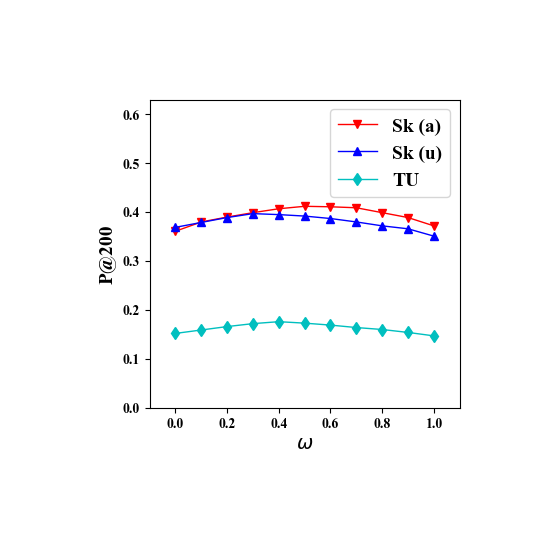
\includegraphics[width=1\linewidth]{omega_fig.pdf}
\end{center}
   \caption{The performance variety along with the $\omega$}
\label{fig:omega}
\end{figure}

\begin{figure}
\begin{center}
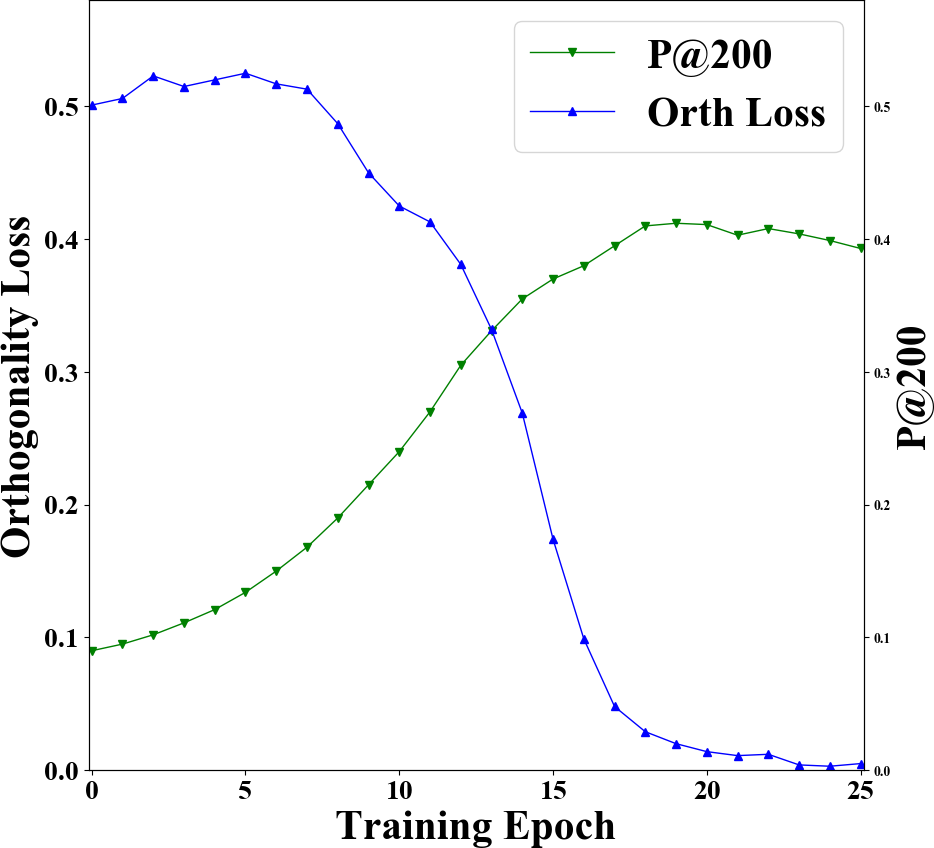
\includegraphics[width=1\linewidth]{orth.pdf}
\end{center}
   \caption{The performance and orthogonality variety along with the training epoch}
\label{fig:orth}
\end{figure}


%\begin{figure}[htbp]
%\centering
%\subfigure 1 {
%\begin{minipage}[t]{0.40\linewidth}
%\centering
%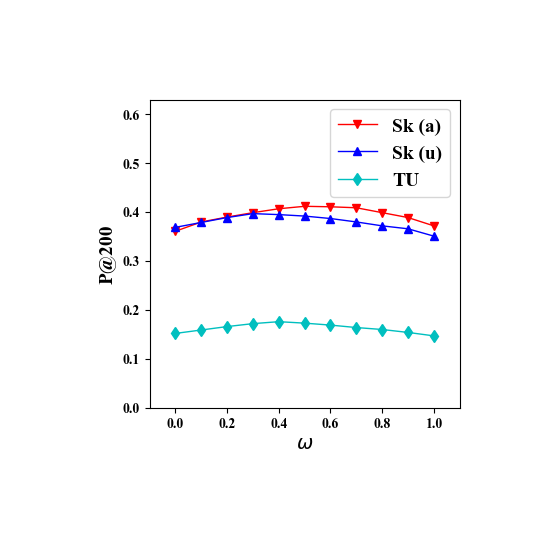
\includegraphics[width=1\linewidth]{omega_fig.pdf}
%\caption{}
%\label{fig:omega}
%\end{minipage}%
%}%
%\subfigure 2 {
%\begin{minipage}[t]{0.45\linewidth}
%\centering
%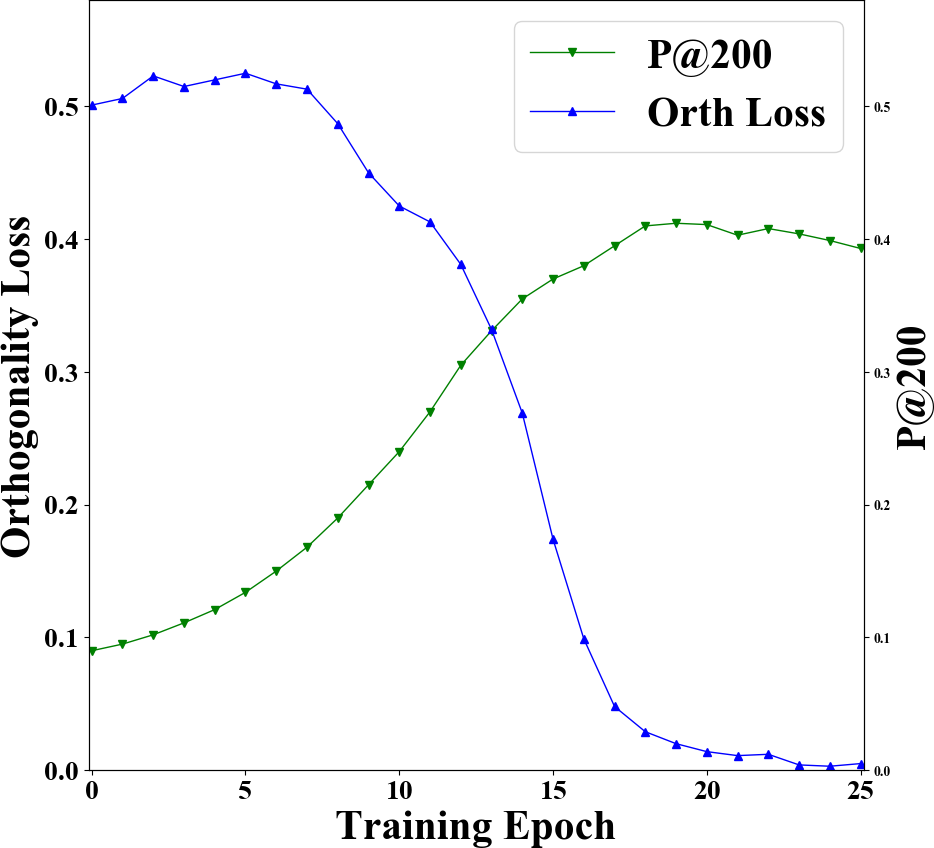
\includegraphics[width=1\linewidth]{orth.pdf}
%\caption{}
%\label{fig:orth}
%\end{minipage}%
%}
%\centering
%\caption{1. The performance variety along with the $\omega$; 2. The performance and orthogonality variety along with the training epoch }
%\end{figure}


\subsection{Ablation Study}
We analyze the effect of different loss functions, some alternations while designing the model and the effect of $\omega$ on Sketchy Ext dataset.

\noindent\textbf{Loss Analysis}
In Table \ref{tab:2}, we can find the effect of different losses. As expected, the ranking loss and the image reconstruction loss are the most important constrains in our model, which is because these two losses mainly control the image-sketch distance in their corresponding space. Besides, the image reconstruction loss has bigger effect on aligned data than that on unaligned data, which indicated the reconstruction loss is sensitive to the pose information. However, the image adversarial loss have much bigger effect on the unaligned dataset, which shows the adversarial loss can relief the strong constrain bring from image reconstruction loss in unaligned data. 

\noindent\textbf{Alternation Analysis}
In the last two rows, we show two alternations, (1) move the orthogonality loss from ($f_{im}^{ap},f_{im}^{st}$) to ($z_{im}^{ap},f_{im}^{st}$) and (2) directly translate the image from the sketch structure feature without the image appearance feature $z_{im}^{ap}$. The performance drop after moving the orthogonality loss to $z_{im}^{ap}$ and $f_{im}^{st}$, which indicate the effect of the disentangled representation. Besides, the performance also drop after we remove the variational estimator, which show the uncertainty compensation is crucial to train the image generator.

\noindent\textbf{Retrieval Strategy  Analysis}
In Figure \ref{fig:omega}, we plot the $\omega$-P@200 curve. From this figure, we can find that the optimal $\omega$ is between $0.4$ and $0.6$. \color{red}Besides, the peak of the curve usually close to the retrieval space who have higher performance.\color{black}

\subsection{Disentangle Analysis}
To prove that our model actually disentangles the image features into structure space and appearance space, we first plot the varity of orthogonality loss and P@200 during the training and then \color{red}we visualize the all the image and sketch features\color{black} using t-SNE \cite{maaten2008visualizing}.

As you can see in Figure \ref{fig:orth}, the orthogonality loss drops very slow at the first 6 training epoch. But during the 7-16 training epoch, the orthogonality loss drops very quickly. Compared with the variety of P@200, we find the similar tendency which indicates that the image disentanglement help our proposed model to generalize from seen to unseen categories in a great deal.

\begin{figure}
\begin{center}
\includegraphics[width=1\linewidth]{tsne.pdf}
\end{center}
   \caption{t-SNE results for different features on the testing set of Sketchy Ext. This figure is best viewed in color.}
\label{fig:tsne}
\end{figure}

In Figure \ref{fig:tsne}, we show the t-SNE results on image features, image appearance features, image structure features, sketch features, sketch structure features, sketch translated image features. From these figures we can find that the image feature is well disentangled into structure feature and appearance, \color{red}in which the image appearance is cluster as different cycle in different appearance.\color{black} Besides, the cluster results between image feature and translated image feature are similar and the cluster results between image structure feature and sketch structure feature are also similar, which also shows better alignment.

\begin{figure}
\begin{center}
\includegraphics[width=1\linewidth]{casestudy.pdf}
\end{center}
   \caption{The top-5 images retrieved among BDT, BDT-St, BDT-Im, CVAE on Sketchy Ext. (Aligned) dataset. The green border indicates the right retrieval results and the red border indicates the opposite.}
\label{fig:case}
\end{figure}

\subsection{Case study}
In Figure \ref{fig:case}, we show the retrieval results of \textbf{BDT-St}, \textbf{BDT-Im}, \textbf{BDT} and CVAE \cite{yelamarthi2018zero}. Comparing them, we can find that the retrieval results in structure feature space concern more about the outlines and the retrieval results in image feature space care more about the pose and detailed features, which is similar to the results of CVAE, eg, for the sketch $door$, the retrieval results of both CVAE and BDT-Im have the $grid$, the results of BDT-St only contains the general outlines of $doorcase$.

\section{Conclusion}
This paper studies the problem of zero-shot sketch-based image retrieval from a new point of view, aka, using disentangled representation to facilitate the structure-based retrieval. To integrate the disentangled representation into a retrieval model, we proposed Bi-directional Domain Translation framework (BDT) in this paper and perform retrieval from two features space. Experiments on both Sketchy Ext. (aligned/unaligned) and TU-Berlin Ext. dataset demonstrate state-of-the-art performance. In further analysis and case study, we prove the model is capable of disentangling structure and appearance features for the image and the disentangled representation is indeed helpful for our model to generalize from seen categories to unseen categories.


{\small
\bibliographystyle{ieee_fullname}
\bibliography{egbib}
}

\end{document}
